



\begin{figure*}[t]
\centering
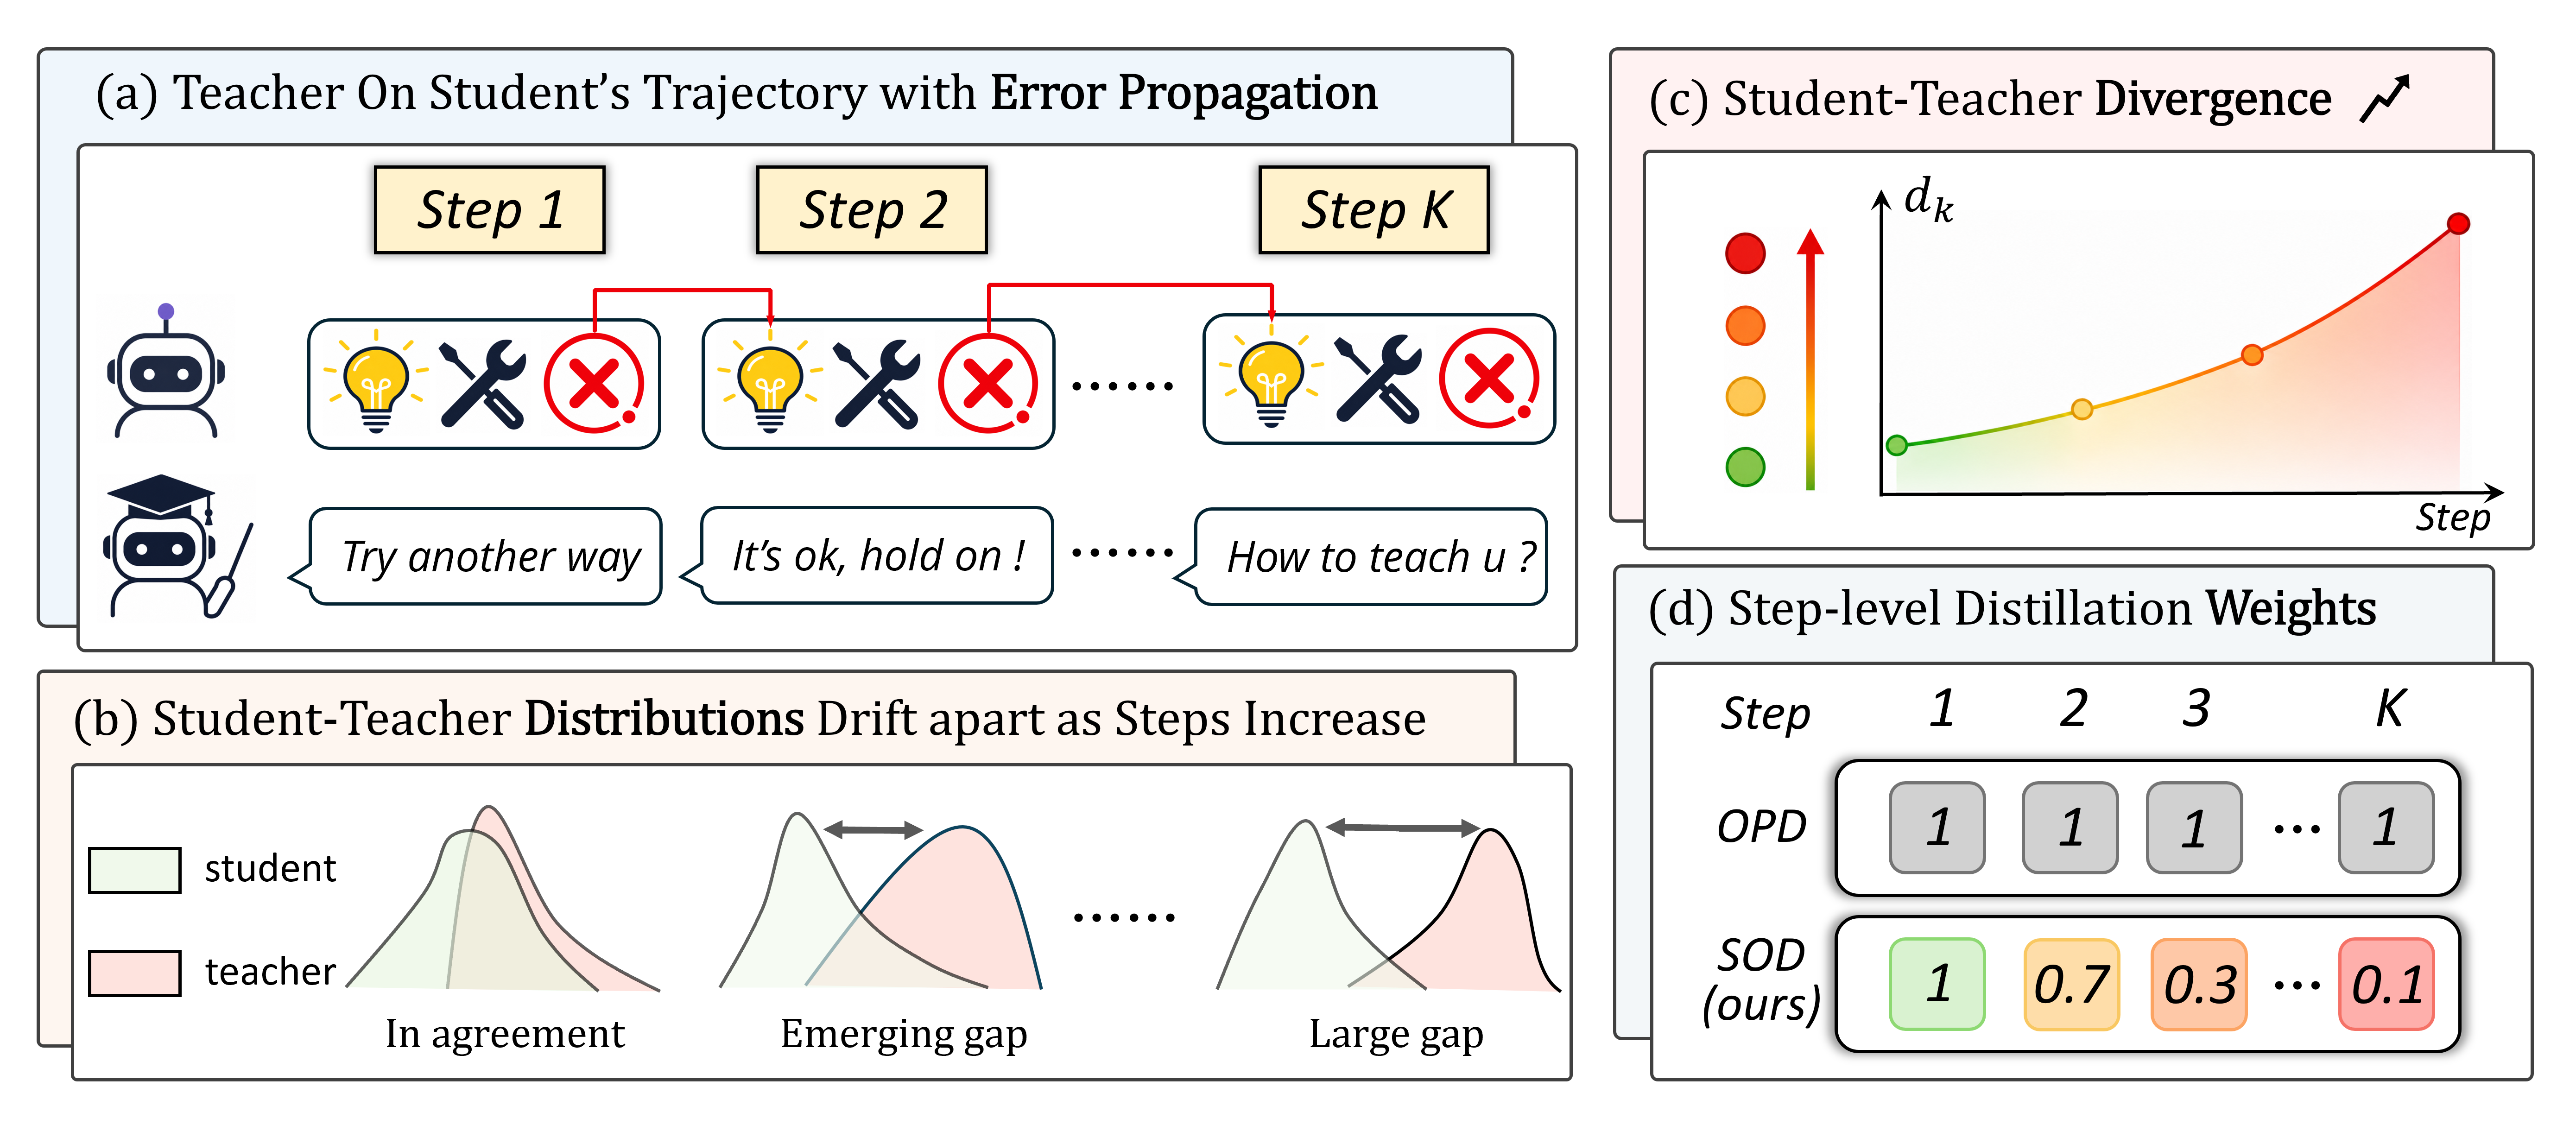
\includegraphics[width=1.0\linewidth]{pic/framework7.png}
\caption{\textbf{The overview of \ourmodel}. (a)~The student generates multi-step trajectories where erroneous tool calls propagate across steps, degrading teacher supervision reliability. (b)~Student-teacher distributions drift apart as errors accumulate. (c)~Step-level divergence $d_k$ quantifies this drift. (d)~\ourmodel adaptively attenuates distillation weights in high-divergence steps, unlike vanilla OPD which applies uniform weights. Please refer to~\cref{rq5_body} for more characteristics of \ourmodel.}
\label{framework}
 \vspace{-0.09 in}
\end{figure*}




\subsection{Student-teacher Divergence and Step-wise Reweighting}

We partition a generated trajectory into $K+1$ reasoning steps, where each step corresponds to a model response between two tool observations, or the final answer step. Let $\mathcal{I}_k$ denote the set of token positions belonging to the $k$-th model-generated step. Tool observation tokens are excluded because they are produced by the external environment rather than by the policy.

We define a step-level divergence score to quantify student–teacher divergence at step $k$:

\begin{equation}
    d_k =
    \frac{1}{|\mathcal{I}_k|}
    \sum_{t \in \mathcal{I}_k}
    \left|
    \log \pi_\theta(y_t \mid y_{<t})
    -
    \log \pi_{\mathrm{teacher}}(y_t \mid y_{<t})
    \right|.
\label{eq:step_div}
\end{equation}


The score $d_k$ serves as a lightweight indicator of the local reliability of teacher supervision. A small $d_k$ suggests that the student remains well aligned with the teacher distribution, while a large $d_k$ indicates substantial mismatch, often caused by tool-induced state drift or corrupted observations. 




Based on these divergence scores, we adaptively reweight the strength of distillation across steps.
We initialize the first step with full distillation strength, \ie $w_1 = 1$. For subsequent steps, the weight is:
\begin{equation}
    w_k =
    \min\!\left(
    w_1
    \prod_{u=1}^{k-1}
    \frac{d_u + \epsilon}{d_{u+1} + \epsilon},
    1 + \delta
    \right),
    \quad k \ge 2,
\label{eq:adaptive_weight}
\end{equation}
where $\epsilon$ is a small constant for stability and $\delta$ controls the maximum amplification of the distillation.
Since the reweighting in~\cref{eq:adaptive_weight} depends only on the \emph{ratios} between consecutive divergence scores rather than their absolute values, any monotone proxy of $\Delta_k$ suffices. We show in~\cref{app:dk_proxy} that $d_k$ is monotonically consistent with $\Delta_k$ and computable at zero marginal cost from the OPD forward pass. We therefore adopt $d_k$ in place of $\Delta_k$ in our implementation.



This weighting rule captures the evolution of student-teacher divergence along the trajectory. When the divergence increases, \ie $d_{u+1} > d_u$, indicating that the student is drifting away from the teacher distribution (often due to tool-induced state shift), the corresponding ratio becomes smaller than one, leading to attenuation of the distillation signal in high-mismatch regions. 
Conversely, the student may partially move back toward the teacher-supported region in later steps, effectively correcting earlier deviations. We refer to this phenomenon as \textit{recovery from earlier errors}. In such cases, when $d_{u+1} < d_u$, the reweighting mechanism allows the distillation strength to increase accordingly, restoring informative guidance. To ensure stable optimization, the weight is upper-bounded by $1+\delta$.





\subsection{Training Objective}

For a student-generated trajectory, the sampled-token OPD term at token $t$ is:
\begin{equation}
    \ell_{\mathrm{OPD}}(y_t)
    =
    \log \pi_\theta(y_t \mid y_{<t})
    -
    \log \pi_{\mathrm{teacher}}(y_t \mid y_{<t}).
\end{equation}

Instead of applying this term uniformly at step level, we reweight all tokens in step $k$ by the corresponding reliability weight $w_k$, leading to the step-wise OPD objective:
\begin{equation}
    \mathcal{L}_{\mathrm{OPD}}^{\mathrm{step}}
    =
    \mathbb{E}_{y \sim \pi_\theta}
    \left[
    \sum_{k=1}^{K+1}
    w_k
    \sum_{t \in \mathcal{I}_k}
    \left(
    \log \pi_\theta(y_t \mid y_{<t})
    -
    \log \pi_{\mathrm{teacher}}(y_t \mid y_{<t})
    \right)
    \right].
\label{eq:step_opd}
\end{equation}

The final training objective is defined as:
\begin{equation}
\label{eq:training_object}
    \mathcal{L}
    =
    \mathcal{L}_{\mathrm{GRPO}}
    +
    \mathcal{L}_{\mathrm{OPD}}^{\mathrm{step}}.
\end{equation}


Here, $\mathcal{L}_{\mathrm{GRPO}}$ provides sparse outcome-level rewards to drive trajectory exploration, while $\mathcal{L}_{\mathrm{OPD}}^{\mathrm{step}}$ supplies dense token-level guidance whose strength is reweighted by the student-teacher divergence, jointly enabling stable learning under tool-induced state drift.
